\section{Empirical Evidence}
\label{sec:empirical}

The empirical exercise is intended to validate the sign and sorting implications of the model, rather than to provide a stand-alone causal estimate of fiscal adaptation spending. The estimates are therefore interpreted as theory-guided reduced-form evidence. The main objects are empirical analogues of the model's spread-relief and debt-improving conditions, constructed from country-year variation in sovereign spreads, public debt, and climate-readiness measures.

\subsection{Data, Proxies, and Measurement Units}

The sample is an unbalanced country-year panel covering 1995--2023. The United States is excluded throughout the empirical analysis. The dependent variable in the spread regressions is the sovereign spread, $s_{it}$. The adaptation-readiness proxy is $G_{it}$, constructed from ND-GAIN readiness performance. The vulnerability-performance proxy is $X_{it}$, constructed from ND-GAIN vulnerability performance. Debt exposure is measured by debt/GDP, $B_{it}$.

The empirical variables are expressed in analysis units. The adaptation proxy $G_{it}$ is constructed from ND-GAIN readiness performance, while $X_{it}$ is constructed from ND-GAIN vulnerability performance. Higher $G_{it}$ indicates stronger improvements in adaptation readiness. Higher $X_{it}$ indicates lower vulnerability relative to GDP-predicted vulnerability. Sovereign spreads, debt ratios, fiscal ratios, and macroeconomic rates are expressed in share units; for these variables, 0.01 corresponds to one percentage point.\footnote{For variables expressed in share units, a one-percentage-point change corresponds to a 0.01 change in the regressor. The tables report coefficients in these analysis units.}

The control vector is denoted by $\mathbf{Z}_{it}=(Z_{1,it},Z_{2,it},\ldots,Z_{8,it})'$. The components are real GDP, real GDP growth, CPI inflation, overall balance/GDP, international reserves, government effectiveness, regulatory quality, and terms of trade. The main regressions include country fixed effects and year fixed effects, and report robust $t$-statistics. Table~\ref{tab:summary_stats} summarizes the post-preprocessing variables used in the analysis.

\begin{table}[H]\centering
\begin{threeparttable}
\caption{Post-Preprocessing Descriptive Statistics}
\label{tab:summary_stats}
\scriptsize
\setlength{\tabcolsep}{2.6pt}
\begin{tabularx}{\textwidth}{llYYYYYY}
\toprule
Block & Variable & $N$ & Mean & SD & Median & Min. & Max. \\
\midrule
$S$ & Sovereign spread & 1,272 & 0.024 & 0.043 & 0.007 & -0.034 & 0.343 \\
$G$ & Readiness performance & 1,798 & 0.058 & 0.089 & 0.048 & -0.326 & 0.303 \\
$B$ & Debt/GDP & 1,712 & 0.586 & 0.342 & 0.522 & 0.039 & 2.610 \\
$X$ & Vulnerability performance & 1,798 & -0.040 & 0.058 & -0.047 & -0.185 & 0.295 \\
$Z_1$ & Real GDP & 1,791 & 0.080 & 0.029 & 0.077 & 0.019 & 0.163 \\
$Z_2$ & Real GDP growth & 1,787 & 0.034 & 0.036 & 0.035 & -0.145 & 0.246 \\
$Z_3$ & CPI inflation & 1,791 & 0.057 & 0.108 & 0.032 & -0.018 & 1.973 \\
$Z_4$ & Overall balance/GDP & 1,697 & -0.004 & 0.034 & -0.005 & -0.300 & 0.234 \\
$Z_5$ & International reserves & 1,753 & 0.055 & 0.128 & 0.018 & 0.000 & 1.527 \\
$Z_6$ & Government effectiveness & 1,550 & 0.006 & 0.009 & 0.007 & -0.013 & 0.025 \\
$Z_7$ & Regulatory quality & 1,550 & 0.006 & 0.008 & 0.007 & -0.013 & 0.023 \\
$Z_8$ & Terms of trade & 1,595 & 1.006 & 0.187 & 0.994 & 0.319 & 2.731 \\
\bottomrule
\end{tabularx}
\begin{tablenotes}[flushleft]\footnotesize
\item Notes: Statistics use the post-preprocessing non-U.S. 1995--2023 panel. Each row is computed on nonmissing observations for the corresponding variable.
\end{tablenotes}
\end{threeparttable}
\end{table}

\subsection{Adaptation and Sovereign Financing Costs}

The baseline spread regression tests the sign prediction in Proposition 2:
\begin{equation}
s_{it}
=
\alpha_i+\tau_t
+\beta_G G_{it}
+\beta_B B_{it}
+\beta_X X_{it}
+\boldsymbol{\Gamma}'\mathbf{Z}_{it}
+u_{it}.
\label{eq:emp_baseline_spread}
\end{equation}
Table~\ref{tab:baseline_spread} provides reduced-form evidence consistent with Proposition 2. The coefficient on $G_{it}$ is negative and statistically significant, indicating that improvements in the adaptation-readiness proxy are associated with lower sovereign financing costs. The coefficient on $B_{it}$ is positive, and the coefficient on $X_{it}$ is negative. Since higher $X_{it}$ means lower vulnerability relative to GDP-predicted vulnerability, this latter coefficient is consistent with lower spreads among countries with better vulnerability performance.

\begin{table}[H]\centering
\begin{threeparttable}
\caption{Baseline Fixed-Effects Estimates}
\label{tab:baseline_spread}
\scriptsize
\begin{tabularx}{0.78\textwidth}{lY}
\toprule
Dependent variable & 10-year sovereign spread, $s_{it}$ \\
\midrule
$G_{it}$ & -0.046*** \\
  & (-2.804) \\
$B_{it}$ & 0.043*** \\
  & (6.042) \\
$X_{it}$ & -0.087*** \\
  & (-2.626) \\
\midrule
Controls $\mathbf{Z}_{it}$ & Yes \\
Country FE & Yes \\
Year FE & Yes \\
Sample period & 1995--2023 \\
Countries & 60 \\
Observations & 1,120 \\
Adjusted $R^2$ & 0.900 \\
\bottomrule
\end{tabularx}
\begin{tablenotes}[flushleft]\footnotesize
\item Notes: Robust $t$-statistics are reported in parentheses. *** $p<0.01$, ** $p<0.05$, * $p<0.10$.
\end{tablenotes}
\end{threeparttable}
\end{table}

\subsection{Heterogeneous Spread Relief and the Empirical Debt-Improving Index}

The next step asks whether the spread-relief effect of the readiness-performance proxy varies with debt exposure and vulnerability performance, as suggested by Corollary 1. The full-interaction spread model is
\begin{equation}
s_{it}
=
\alpha_i+\tau_t
+\beta_GG_{it}
+\beta_BB_{it}
+\beta_XX_{it}
+\beta_{GB}(G_{it}\times B_{it})
+\beta_{GX}(G_{it}\times X_{it})
+\boldsymbol{\Gamma}'\mathbf{Z}_{it}
+u_{it}.
\label{eq:emp_full_interaction_spread}
\end{equation}
For the empirical index construction, the expanded full-interaction specification also allows the marginal effect of $G_{it}$ to vary with the control vector:
\begin{equation}
\begin{aligned}
s_{it}
&=
\alpha_i+\tau_t
+\beta_GG_{it}
+\beta_BB_{it}
+\beta_XX_{it} \\
&\quad
+\beta_{GB}(G_{it}\times B_{it})
+\beta_{GX}(G_{it}\times X_{it})
+\boldsymbol{\Pi}'(G_{it}\times\mathbf{Z}_{it})
+\boldsymbol{\Gamma}'\mathbf{Z}_{it}
+u_{it}.
\end{aligned}
\label{eq:emp_full_interaction_spread_gz}
\end{equation}
Here, $G_{it}\times\mathbf{Z}_{it}$ denotes the vector of interactions between $G_{it}$ and each component of $\mathbf{Z}_{it}$. The implied marginal effect of $G_{it}$ in equation~\eqref{eq:emp_full_interaction_spread_gz} is
\begin{equation}
\frac{\partial s_{it}}{\partial G_{it}}
=
\beta_G
+\beta_{GB}B_{it}
+\beta_{GX}X_{it}
+\boldsymbol{\Pi}'\mathbf{Z}_{it}.
\label{eq:emp_marginal_spread}
\end{equation}
The implied marginal spread relief and empirical debt-improving index are
\begin{equation}
\widehat m^{G,F}_{it}
=
-
\frac{\partial \widehat s_{it}}{\partial G_{it}},
\qquad
\widehat\theta^F_{it}
=
B_{it}\widehat m^{G,F}_{it}.
\label{eq:emp_theta}
\end{equation}
The index $\widehat\theta^F_{it}$ should be interpreted as an empirical proxy for debt-improving capacity, not as a structural estimate of the theoretical $\theta_t$.

Table~\ref{tab:heterogeneity_spread} estimates whether the spread-relief effect of the adaptation proxy varies with debt exposure and vulnerability performance. The negative coefficient on $G_{it}\times B_{it}$ indicates that spread relief is stronger at higher debt levels. Because $X_{it}$ is a vulnerability-performance measure, higher values indicate lower vulnerability relative to GDP-predicted vulnerability. Therefore, stronger marginal relief at lower $X_{it}$ should be interpreted as stronger spread relief among more vulnerable countries. Table~\ref{tab:theta_stats} then uses the expanded full-interaction specification to summarize the empirical debt-improving index, $\widehat\theta^F_{it}=B_{it}\widehat m^{G,F}_{it}$.

\begin{table}[H]\centering
\begin{threeparttable}
\caption{Heterogeneous Spread Relief}
\label{tab:heterogeneity_spread}
\scriptsize
\setlength{\tabcolsep}{3.0pt}
\begin{tabularx}{\textwidth}{lYYYY}
\toprule
Dependent variable & \multicolumn{4}{c}{10-year sovereign spread, $s_{it}$} \\
\midrule
$G_{it}$ & 0.053** & -0.046*** & 0.058** & 0.319*** \\
  & (2.116) & (-2.791) & (2.271) & (4.651) \\
$B_{it}$ & 0.062*** & 0.044*** & 0.064*** & 0.070*** \\
  & (6.922) & (6.056) & (6.995) & (7.456) \\
$X_{it}$ & -0.052 & -0.084** & -0.043 & 0.086* \\
  & (-1.562) & (-2.485) & (-1.244) & (1.900) \\
$G_{it}\times B_{it}$ & -0.211*** &  & -0.221*** & -0.266*** \\
  & (-4.795) &  & (-4.892) & (-5.723) \\
$G_{it}\times X_{it}$ &  & 0.121 & 0.268** & 0.339** \\
  &  & (1.196) & (2.302) & (2.255) \\
\midrule
Controls $\mathbf{Z}_{it}$ & Yes & Yes & Yes & Yes \\
$G_{it}\times\mathbf{Z}_{it}$ controls & No & No & No & Yes \\
Country FE & Yes & Yes & Yes & Yes \\
Year FE & Yes & Yes & Yes & Yes \\
Countries & 60 & 60 & 60 & 60 \\
Observations & 1,120 & 1,120 & 1,120 & 1,120 \\
Adjusted $R^2$ & 0.905 & 0.900 & 0.906 & 0.911 \\
\bottomrule
\end{tabularx}
\begin{tablenotes}[flushleft]\footnotesize
\item Notes: Columns 1--4 report debt heterogeneity, vulnerability-performance heterogeneity, full interaction, and full interaction with $G_{it}\times\mathbf{Z}_{it}$, respectively. Robust $t$-statistics are reported in parentheses. *** $p<0.01$, ** $p<0.05$, * $p<0.10$.
\end{tablenotes}
\end{threeparttable}
\end{table}

\begin{table}[H]\centering
\begin{threeparttable}
\caption{Empirical Debt-Improving Index Descriptive Statistics}
\label{tab:theta_stats}
\scriptsize
\setlength{\tabcolsep}{3.0pt}
\begin{tabularx}{0.88\textwidth}{lYYYYYY}
\toprule
Variable & $N$ & Mean & SD & Median & Min. & Max. \\
\midrule
$\widehat{\theta}^{F}_{it}$ & 1,120 & 0.062 & 0.151 & 0.020 & -0.094 & 1.285 \\
$\widehat m^{G,F}_{it}$ & 1,120 & 0.056 & 0.106 & 0.044 & -0.184 & 0.562 \\
$\partial \widehat s_{it}/\partial G_{it}$ & 1,120 & -0.056 & 0.106 & -0.044 & -0.562 & 0.184 \\
\bottomrule
\end{tabularx}
\begin{tablenotes}[flushleft]\footnotesize
\item Notes: Statistics are computed on the expanded full-interaction spread-model estimation sample. The marginal relief variable is $\widehat m^{G,F}_{it}= -\partial \widehat s_{it}/\partial G_{it}$, and the empirical debt-improving index is $\widehat\theta^F_{it}=B_{it}\widehat m^{G,F}_{it}$.
\end{tablenotes}
\end{threeparttable}
\end{table}

\subsection{Visualizing Spread Relief and the Empirical Index}

Figure~\ref{fig:spread_relief} plots the implied marginal spread relief,
\[
-
\frac{\partial \widehat s_{it}}{\partial G_{it}},
\]
from the full-interaction specification. Panel A varies debt/GDP while holding vulnerability performance at its median. Panel B varies vulnerability performance while holding debt/GDP at its median. The confidence intervals are delta-method intervals based on the robust variance-covariance matrix of $(\widehat{\beta}_G,\widehat{\beta}_{GB},\widehat{\beta}_{GX})$.

\begin{figure}[H]\centering
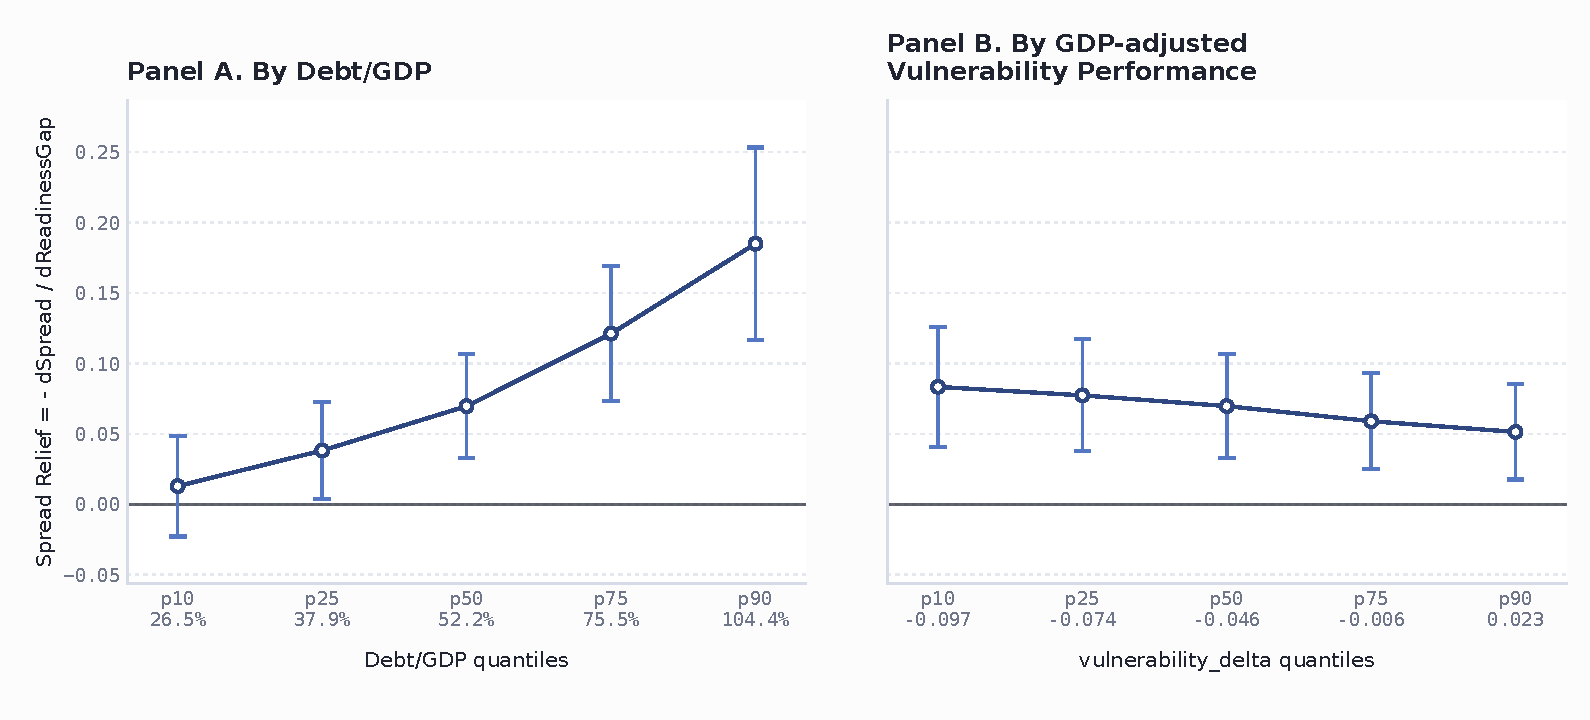
\includegraphics[width=\textwidth]{../best2/result/figure2.pdf}
\caption{Marginal Spread Relief from the Full-Interaction Spread Model}
\label{fig:spread_relief}
\begin{minipage}{0.96\textwidth}
\footnotesize
\textit{Notes:} Panel A fixes $X_{it}$ at its median. Panel B fixes $B_{it}$ at its median. Higher $X_{it}$ indicates lower vulnerability relative to GDP-predicted vulnerability, so the downward slope in Panel B indicates stronger spread relief among more vulnerable observations.
\end{minipage}
\end{figure}

Figure~\ref{fig:theta_distribution} plots the country-year distribution of $\widehat\theta^F_{it}$ and country-level average rankings. The dashed line marks the preferred empirical cutoff selected by the kink specification below. It should not be interpreted as the theoretical threshold $\theta_t=1$.

\begin{figure}[H]\centering
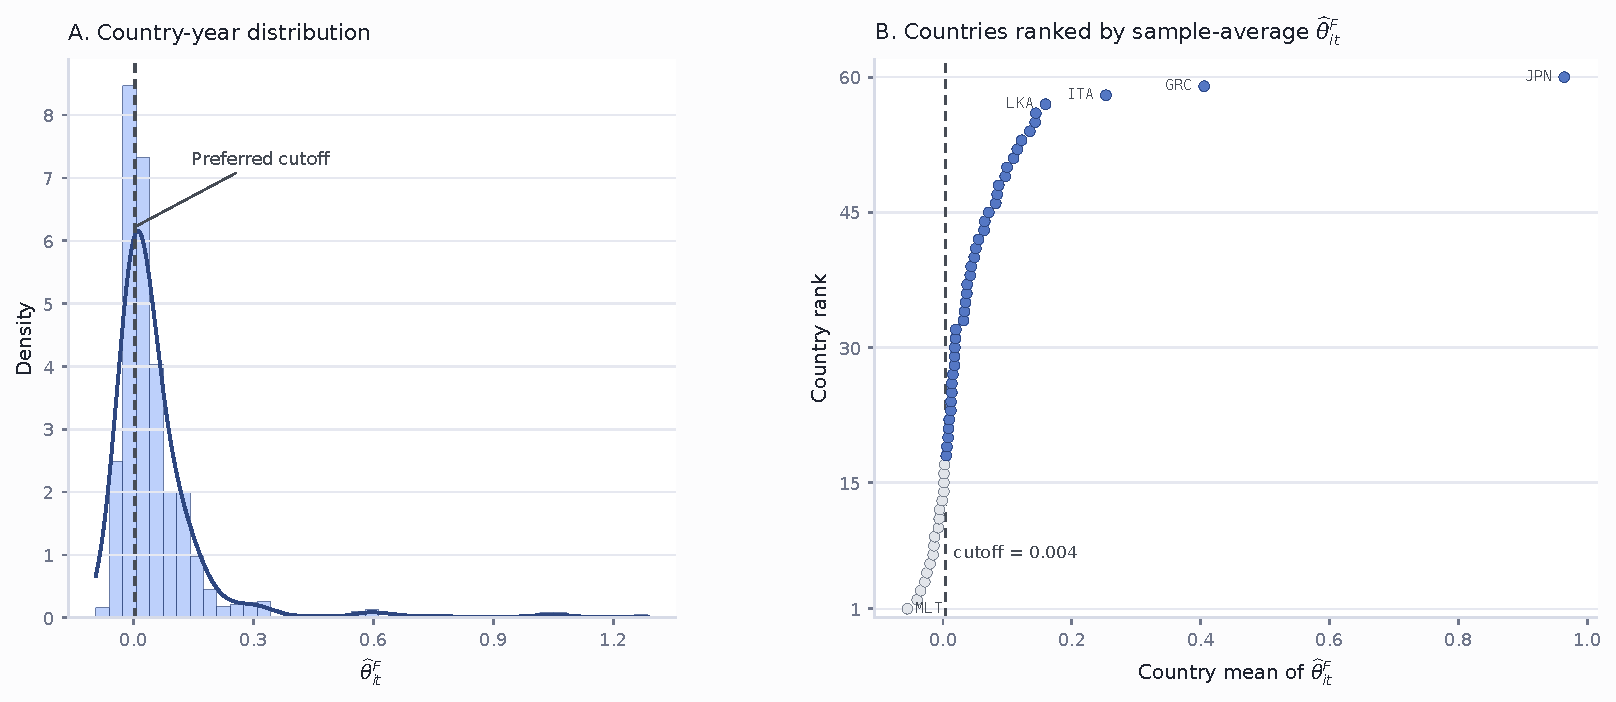
\includegraphics[width=\textwidth]{../best2/result/figure1_theta_distribution_cutoff.pdf}
\caption{Distribution of the Empirical Debt-Improving Index}
\label{fig:theta_distribution}
\begin{minipage}{0.96\textwidth}
\footnotesize
\textit{Notes:} The left panel plots the country-year distribution of $\widehat\theta^F_{it}$. The right panel ranks countries by sample-average $\widehat\theta^F_{it}$. The dashed line marks the preferred empirical cutoff from the without-theta-controls kink specification.
\end{minipage}
\end{figure}

\subsection{Debt Dynamics and the Continuous Theta Interaction}

The next set of tests asks whether the readiness-performance proxy is associated with next-period debt changes in a way that varies with the empirical debt-improving index. Define
\begin{equation}
\Delta B_{i,t+1}
=
B_{i,t+1}-B_{it}.
\label{eq:emp_deltaB}
\end{equation}
The baseline debt-change regression is
\begin{equation}
\Delta B_{i,t+1}
=
\alpha_i+\tau_t
+\lambda_0G_{it}
+\boldsymbol{\Gamma}'\mathbf{Z}_{it}
+\varepsilon_{it},
\label{eq:emp_debt_baseline}
\end{equation}
and the continuous theta interaction model is
\begin{equation}
\Delta B_{i,t+1}
=
\alpha_i+\tau_t
+\lambda_0G_{it}
+\lambda_1(G_{it}\times\widehat\theta^F_{it})
+\boldsymbol{\Gamma}'\mathbf{Z}_{it}
+\varepsilon_{it}.
\label{eq:emp_debt_theta}
\end{equation}
Table~\ref{tab:debt_change} asks whether the marginal effect of the adaptation-readiness proxy on next-period debt changes varies with the empirical debt-improving index. The negative coefficient on $G_{it}\times \widehat\theta^F_{it}$ indicates that higher debt-improving capacity is associated with a lower marginal effect of readiness improvements on debt accumulation. This is consistent with Corollary 4, but it should not be read as evidence that high-theta countries mechanically reduce debt in every case.

\begin{table}[H]\centering
\begin{threeparttable}
\caption{Debt-Change Regressions}
\label{tab:debt_change}
\scriptsize
\setlength{\tabcolsep}{3.0pt}
\begin{tabularx}{\textwidth}{lYYY}
\toprule
Dependent variable & \multicolumn{3}{c}{$\Delta B_{i,t+1}=B_{i,t+1}-B_{it}$} \\
\midrule
$G_{it}$ & -0.073 & -0.042 & -0.015 \\
 & (-1.463) & (-0.810) & (-0.302) \\
$G_{it}\times\widehat\theta^F_{it}$ &  & -0.886*** & -0.310 \\
 &  & (-2.707) & (-0.660) \\
$\widehat\theta^F_{it}$ &  &  & -0.141* \\
 &  &  & (-1.898) \\
Real GDP & 8.143*** & 7.869*** & 5.352*** \\
 & (5.436) & (5.370) & (2.977) \\
Real GDP growth & -0.342*** & -0.346*** & -0.392*** \\
 & (-3.715) & (-3.796) & (-4.179) \\
CPI inflation & -0.173** & -0.174** & -0.158** \\
 & (-2.053) & (-2.060) & (-2.070) \\
Overall balance/GDP & -0.480*** & -0.458*** & -0.416*** \\
 & (-6.090) & (-5.862) & (-5.204) \\
International reserves & 0.018 & 0.020 & 0.019 \\
 & (1.299) & (1.456) & (1.366) \\
Government effectiveness & -1.777* & -1.396 & -0.601 \\
 & (-1.895) & (-1.470) & (-0.575) \\
Regulatory quality & 1.637* & 0.815 & -0.405 \\
 & (1.857) & (0.907) & (-0.404) \\
Terms of trade & 0.044*** & 0.037** & 0.037*** \\
 & (2.845) & (2.484) & (2.584) \\
\midrule
Theta main effect & No & No & Yes \\
Controls $\mathbf{Z}_{it}$ & Yes & Yes & Yes \\
Country FE & Yes & Yes & Yes \\
Year FE & Yes & Yes & Yes \\
Observations & 1,060 & 1,060 & 1,060 \\
Countries & 60 & 60 & 60 \\
Adjusted $R^2$ & 0.425 & 0.433 & 0.441 \\
\bottomrule
\end{tabularx}
\begin{tablenotes}[flushleft]\footnotesize
\item Notes: Columns 1--3 report the baseline model, the continuous theta interaction model, and the full-theta dynamics model, respectively. The full-theta dynamics specification includes $\widehat\theta^F_{it}$ as a direct control. Robust $t$-statistics are reported in parentheses. *** $p<0.01$, ** $p<0.05$, * $p<0.10$.
\end{tablenotes}
\end{threeparttable}
\end{table}

\subsection{Grouped Debt-Change Heterogeneity}

Table~\ref{tab:grouped_debt_change} compares three ways of sorting the sample: by the composite debt-improving index $\widehat\theta^F_{it}$, by debt/GDP $B_{it}$, and by marginal spread relief $\widehat m^{G,F}_{it}$. Panel A shows that the coefficient on $G_{it}$ turns from positive in low-$\widehat\theta$ groups to negative in high-$\widehat\theta$ groups. Panel B shows that sorting by debt/GDP alone does not generate the same clear pattern. Panel C shows a similar ordering when observations are sorted by marginal spread relief, but this sorting omits the debt-exposure component that is central to the theoretical index. Overall, the comparison supports the theoretical composite object $B_{it}\widehat m^{G,F}_{it}$, rather than debt exposure alone, as the relevant empirical sorting variable for debt dynamics.

\begin{table}[H]\centering
\caption{Grouped Debt-Change Heterogeneity Regressions}
\label{tab:grouped_debt_change}
\begin{threeparttable}
\scriptsize
\setlength{\tabcolsep}{3.0pt}
\renewcommand{\arraystretch}{1.10}
\textbf{Panel A. Full-theta groups}\\[0.45em]
\begin{tabularx}{\textwidth}{lYYYYY}
\toprule
Dependent variable & \multicolumn{5}{c}{$B_{i,t+1}-B_{it}$} \\
\cmidrule(lr){2-6}
Group & 0--20\% & 20--40\% & 40--60\% & 60--80\% & 80--100\% \\
\midrule
$G_{it}$ & 0.243* & 0.057 & -0.152 & -0.249* & -0.372** \\
 & (1.727) & (0.866) & (-1.550) & (-1.770) & (-2.077) \\
\midrule
Controls $\mathbf{Z}_{it}$ & Yes & Yes & Yes & Yes & Yes \\
Country FE & Yes & Yes & Yes & Yes & Yes \\
Year FE & Yes & Yes & Yes & Yes & Yes \\
Observations & 212 & 212 & 212 & 212 & 212 \\
Countries & 25 & 33 & 35 & 37 & 22 \\
Adjusted $R^2$ & 0.604 & 0.669 & 0.499 & 0.366 & 0.522 \\
\bottomrule
\end{tabularx}

\vspace{0.75em}
\textbf{Panel B. Debt-ratio groups}\\[0.45em]
\begin{tabularx}{\textwidth}{lYYYYY}
\toprule
Dependent variable & \multicolumn{5}{c}{$B_{i,t+1}-B_{it}$} \\
\cmidrule(lr){2-6}
Group & 0--20\% & 20--40\% & 40--60\% & 60--80\% & 80--100\% \\
\midrule
$G_{it}$ & 0.060 & -0.116 & -0.067 & 0.038 & -0.363 \\
 & (0.861) & (-1.336) & (-1.021) & (0.291) & (-1.317) \\
\midrule
Controls $\mathbf{Z}_{it}$ & Yes & Yes & Yes & Yes & Yes \\
Country FE & Yes & Yes & Yes & Yes & Yes \\
Year FE & Yes & Yes & Yes & Yes & Yes \\
Observations & 212 & 212 & 212 & 212 & 212 \\
Countries & 28 & 35 & 41 & 32 & 22 \\
Adjusted $R^2$ & 0.466 & 0.483 & 0.700 & 0.394 & 0.625 \\
\bottomrule
\end{tabularx}

\vspace{0.75em}
\textbf{Panel C. Marginal-relief groups}\\[0.45em]
\begin{tabularx}{\textwidth}{lYYYYY}
\toprule
Dependent variable & \multicolumn{5}{c}{$B_{i,t+1}-B_{it}$} \\
\cmidrule(lr){2-6}
Group & 0--20\% & 20--40\% & 40--60\% & 60--80\% & 80--100\% \\
\midrule
$G_{it}$ & 0.325** & 0.097 & -0.041 & -0.134 & -0.512*** \\
 & (2.244) & (0.732) & (-0.426) & (-1.350) & (-3.273) \\
\midrule
Controls $\mathbf{Z}_{it}$ & Yes & Yes & Yes & Yes & Yes \\
Country FE & Yes & Yes & Yes & Yes & Yes \\
Year FE & Yes & Yes & Yes & Yes & Yes \\
Observations & 212 & 212 & 212 & 212 & 212 \\
Countries & 25 & 36 & 36 & 34 & 24 \\
Adjusted $R^2$ & 0.603 & 0.568 & 0.518 & 0.606 & 0.493 \\
\bottomrule
\end{tabularx}
\begin{tablenotes}[flushleft]\footnotesize
\item Notes: Each column estimates the next-period change in debt/GDP on current GDP-adjusted readiness performance, $G_{it}$, within the indicated subgroup. Macro control coefficients and subgroup cutoff values are omitted for compactness. Robust $t$-statistics are reported in parentheses. *** $p<0.01$, ** $p<0.05$, * $p<0.10$.
\end{tablenotes}
\end{threeparttable}
\end{table}

\subsection{Single-Crossing Kink Test}

The single-crossing specification provides the closest empirical analogue to Corollary 4 and its mirror image. It directly tests whether the marginal effect of the adaptation-readiness proxy on next-period debt changes switches sign around an empirical cutoff. This specification is not a standard panel threshold model. It is designed to estimate whether the marginal debt effect of $G_{it}$ crosses zero as a function of $\widehat\theta^F_{it}$.

For a candidate cutoff $c$, the estimated specification is
\begin{equation}
\Delta B_{i,t+1}
=
\alpha_i+\tau_t
+aG_{it}(c-\widehat\theta^F_{it})_+
+bG_{it}(\widehat\theta^F_{it}-c)_+
+\boldsymbol{\Gamma}'\mathbf{Z}_{it}
+\varepsilon_{it}.
\label{eq:emp_kink}
\end{equation}
The implied marginal effect is
\begin{equation}
m(\theta;c)
=
a(c-\theta)_+
+
b(\theta-c)_+.
\label{eq:emp_kink_marginal}
\end{equation}
The theoretical sign pattern is
\[
a>0,
\qquad
b<0.
\]

Table~\ref{tab:kink_model} selects an empirical cutoff of $c=0.004123$ in the main without-theta-controls specification. Below the cutoff, the estimated marginal effect is positive, consistent with debt-worsening adaptation. Above the cutoff, the estimated marginal effect is negative, consistent with debt-improving adaptation. Because the empirical objects are proxy-scaled, the estimated cutoff should be interpreted as an empirical index boundary rather than the literal theoretical threshold $\theta_t=1$. Appendix~\ref{appendixB} reports additional control-set variants and specifications with direct theta controls.

\begin{table}[H]\centering
\begin{threeparttable}
\caption{Single-Crossing Kink Marginal-Effect Model}
\label{tab:kink_model}
\scriptsize
\setlength{\tabcolsep}{3.0pt}
\begin{tabularx}{0.78\textwidth}{lY}
\toprule
Dependent variable & $B_{i,t+1}-B_{it}$ \\
\midrule
$G_{it}(c-\widehat\theta^F_{it})_+$ & 3.380*** \\
 & (2.592) \\
$G_{it}(\widehat\theta^F_{it}-c)_+$ & -0.804** \\
 & (-2.464) \\
\midrule
Cutoff $c$ & 0.004 \\
RSS & 1.951 \\
Share below cutoff & 0.350 \\
Selection rule & RSS minimum; sign-consistent \\
Controls $\mathbf{Z}_{it}$ & Yes \\
Country FE & Yes \\
Year FE & Yes \\
Observations & 1,060 \\
Adjusted $R^2$ & 0.435 \\
\bottomrule
\end{tabularx}
\begin{tablenotes}[flushleft]\footnotesize
\item Notes: The exact RSS-selected cutoff is $c=0.0041231435658208$. The model includes country and year fixed effects and $\mathbf{Z}_{it}$ controls, but does not include direct theta controls. Robust $t$-statistics are reported in parentheses. *** $p<0.01$, ** $p<0.05$.
\end{tablenotes}
\end{threeparttable}
\end{table}

Figure~\ref{fig:kink_marginal_effect} plots the continuous marginal-effect curve implied by equation~\eqref{eq:emp_kink_marginal}. The left side of the cutoff corresponds to the debt-worsening region, while the right side corresponds to the debt-improving region.

\begin{figure}[H]\centering
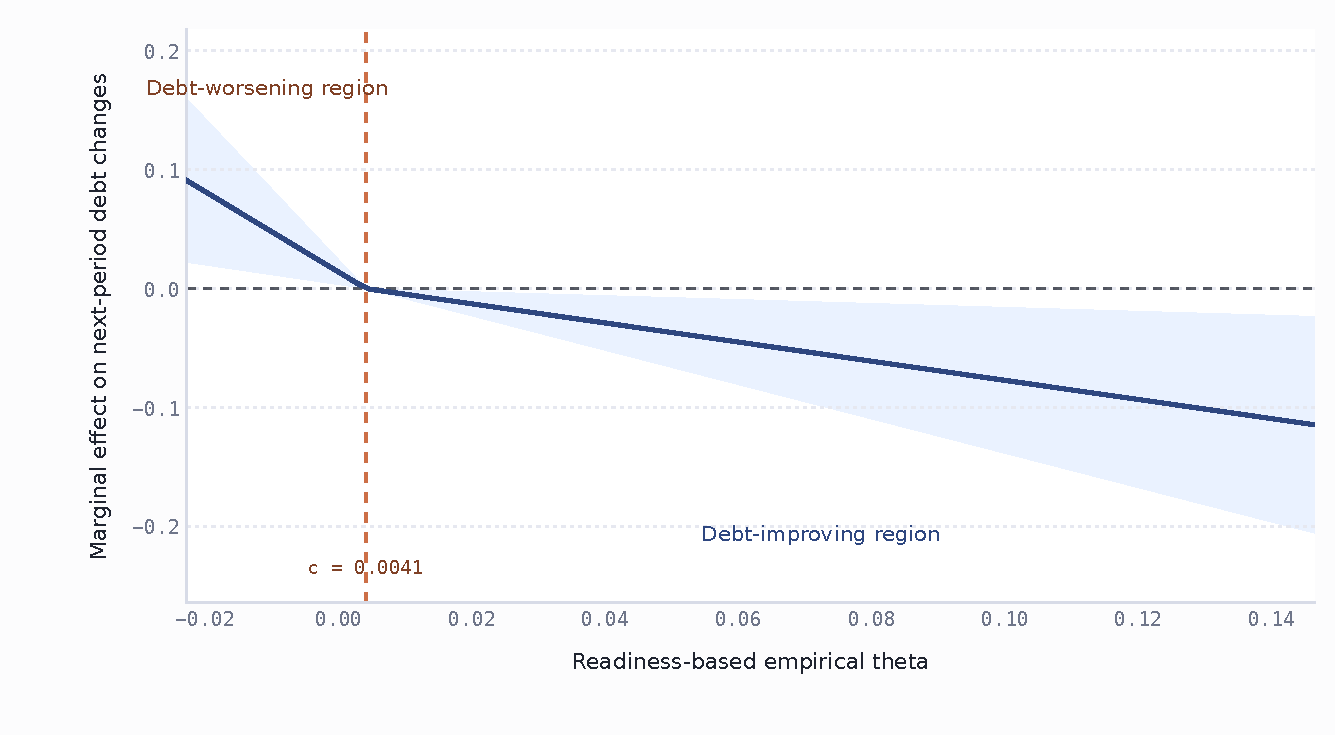
\includegraphics[width=0.92\textwidth]{../best2/result/figure3_kink_marginal_effect_notheta_continuous.pdf}
\caption{Continuous Kink Marginal Effect without Theta Controls}
\label{fig:kink_marginal_effect}
\begin{minipage}{0.92\textwidth}
\footnotesize
\textit{Notes:} The figure plots $m(\theta;c)=a(c-\theta)_+ + b(\theta-c)_+$ from the single-crossing kink model without theta controls. Positive values imply that readiness improvements are associated with higher next-period debt changes; negative values imply lower next-period debt changes. The vertical dashed line marks the empirical cutoff $c$.
\end{minipage}
\end{figure}

\subsection{Country Screens Around the Preferred Cutoff}

Finally, Table~\ref{tab:country_screens} translates the preferred empirical cutoff into an illustrative country-level screen. This exercise is descriptive rather than classificatory. It shows which countries are persistently located on the high-relief or low-relief side of the empirical index. The country screen should be read as a diagnostic application of the empirical index, not as a structural country typology. Vietnam, Indonesia, and Colombia appear as low-debt, high-relief cases under the screening rule, while Malta appears as a high-debt, low-relief case.

\begin{table}[H]\centering
\begin{threeparttable}
\caption{Country Screens Around the Preferred Cutoff}
\label{tab:country_screens}
\scriptsize
\setlength{\tabcolsep}{3.0pt}
\textbf{Panel A. Low debt, theta always above the cutoff, and top-quartile marginal relief}\\[0.45em]
\begin{tabularx}{\textwidth}{llYYYYY}
\toprule
Country & ISO3 & Sample period & Years & Mean debt/GDP & Mean theta & Mean $\widehat m^{G,F}$ \\
\midrule
Vietnam & VNM & 2007--2023 & 17 & 39.50\% & 0.065 & 0.164 \\
Indonesia & IDN & 2003--2023 & 21 & 33.72\% & 0.055 & 0.156 \\
Colombia & COL & 2002--2023 & 21 & 45.82\% & 0.064 & 0.134 \\
\bottomrule
\end{tabularx}

\vspace{0.75em}
\textbf{Panel B. High debt, theta always below the cutoff, and bottom-quartile marginal relief}\\[0.45em]
\begin{tabularx}{\textwidth}{llYYYYY}
\toprule
Country & ISO3 & Sample period & Years & Mean debt/GDP & Mean theta & Mean $\widehat m^{G,F}$ \\
\midrule
Malta & MLT & 2010--2023 & 14 & 53.91\% & -0.055 & -0.107 \\
\bottomrule
\end{tabularx}
\begin{tablenotes}[flushleft]\footnotesize
\item Notes: The preferred cutoff is $c=0.004123$. Screening thresholds use country-level means: the mean-debt median is 53.06 percent, the bottom quartile of mean $\widehat m^{G,F}_{it}$ is 0.003, and the top quartile is 0.112. The always-above and always-below conditions are evaluated year by year.
\end{tablenotes}
\end{threeparttable}
\end{table}
